\subsection{Loop antenna}\label{sec:loop_sim}
\subsubsection{Setup}

\FloatBarrier

\begin{figure}[htbp]
	\centering
	\begin{subfigure}[t]{0.48\textwidth}
		\centering
		\includegraphics[width=1\linewidth]{content/img/loop_near_field}
		\caption{TODO: Maybe show E-Field instead}
		\label{fig:loopnearfield}
	\end{subfigure}
	\hfill
	\begin{subfigure}[t]{0.48\textwidth}
		\centering
		\includegraphics[width=1\linewidth]{content/img/loop_antenna}
		\caption{The geometry of the loop antenna assimilates a square with round edges. Each side has a length of 1.6\,mm. The return path leads back to the PEC surface of the TEM cell.}
		\label{fig:loopantenna}
	\end{subfigure}
	
	\caption{}
	\label{fig:loop_moments_phase}
\end{figure}

A square loop antenna is placed in the center of the TEM cell. It consists of four wires with a length of 1.6\,mm each, and it is electrically short for frequencies up to 4.69\,GHz. The square geometry is preferable to a round version in the numerical simulations, as it allows for more accurate meshes and enables a clearer investigation of the resulting dipole moments. 

The normal vector of the loop surface points in x-direction, leading to a maximum coupling with the magnetic field of the TEM-mode. In contrast to the monopole antenna discussed in \autoref{sec:monopole}, a return path for the current exists, which generates a magnetic dipole moment.

\subsubsection{Equivalent dipole moments}

The equivalent dipole moments of the loop antenna are plotted in \autoref{fig:dipole_moments_loop_antenna}. The magnetic dipole moment $\mathbf{m}_\mathrm{m}$ dominates over the electric dipole moment $\mathbf{m}_\mathrm{e}$. Opposed to the case of a monopole antenna, $\mathbf{m}_\mathrm{e}$ and $\mathbf{m}_\mathrm{m}$ demonstrate non-linear behavior over frequency, which is investigated further in \autoref{sec:loop_electrical_characteristics}.

Furthermore, the phases of the powers at the output ports, shown in \autoref{fig:loopphase}, differ from one another. The phase shift in the low-frequency range approaches $\pi$, but gradually decreases with increasing frequency. This agrees with the analysis presented in \autoref{sec:equ-dip-mom}, which predicts a phase shift of $\pi$ when only $\mathbf{m}_\mathrm{m}$ is present, and a reduced phase shift as $\mathbf{m}_\mathrm{e}$ increases, as is the case here.

\begin{figure}[htbp]
	\centering
	\begin{subfigure}[t]{0.5\textwidth}
		\centering
		\includegraphics[width=1\linewidth]{content/img/dipole_moments_loop_antenna.png}
		\caption{The equivalent dipole moments of the loop antenna derived analytically with \crefrange{eqn:ifa_me}{eqn:ifa_mm}. The electric dipole moment $\mathbf{m}_\mathrm{e}$ is weighted with $Z_0$ to enable comparison with $\mathbf{m}_\mathrm{m}$.}
		\label{fig:dipole_moments_loop_antenna}
	\end{subfigure}
	\hfill
	\begin{subfigure}[t]{0.48\textwidth}
		\centering
		\includegraphics[width=1\linewidth]{content/img/loop_phase}
		\caption{Phases of the powers at output ports 1 and 2, derived from the S-parameters, as discussed in \autoref{sec:s-param-data}. The analysis focuses on the phase shift between the two ports, which provides information about the presence of $\mathbf{m}_\mathrm{m}$ and $\mathbf{m}_\mathrm{e}$, as investigated in \autoref{sec:equ-dip-mom}.}
		\label{fig:loopphase}
	\end{subfigure}
	
	\caption{}
	\label{fig:loop_moments_phase}
\end{figure}

\todo[inline]{TODO: Redo magnetic and electric energy plots logarithmic. Check feed and return current.}

\begin{figure}[htbp]
	\centering
	\begin{subfigure}[b]{0.48\textwidth}
		\centering
		\includegraphics[width=1\linewidth]{content/img/loop_opower}
		\caption{Electric field in y-direction $E_\mathrm{y}$ at $x=0, y=b/4, z=\pm l/2$, and power at one output port, derived with the S-parameters in \autoref{eqn:power_antenna}.}
		\label{fig:loopopower}
	\end{subfigure}
	\hfill
	\begin{subfigure}[b]{0.5\textwidth}
		\centering
		\includegraphics[width=1\linewidth]{content/img/loop_opower_comp}
		\caption{Comparison of output power produced by the monopole antenna and its equivalent dipole moments.}
		\label{fig:loopopowercomp}
	\end{subfigure}
	
	\caption{}
	\label{fig:example}
\end{figure}


The power and $E_y$ induced by the loop antenna at the output ports is shown in \autoref{fig:loopopower}, and increases not as steeply as the output power of the monopole antenna exhibited in \autoref{fig:monopoleoutputpower}. This directly correlates with the decrease of $\mathbf{m}_\mathrm{m}$ with increasing frequency.

\autoref{fig:loopopowercomp} demonstrates the output power generated by the equivalent dipole moments $\mathbf{m}_\mathrm{m}$, $\mathbf{m}_\mathrm{e}$ and the loop antenna. Their similarity support the validity of the model used.

\subsubsection{Electrical characteristics}\label{sec:loop_electrical_characteristics}

\begin{figure}[htbp]
	\centering
	\begin{subfigure}[b]{0.45\textwidth}
		\centering
		\includegraphics[width=1\linewidth]{content/img/loop_elec_energy}
		\caption{Electric energy}
		\label{fig:loopelecenergy}
	\end{subfigure}
	\hfill
	\begin{subfigure}[b]{0.45\textwidth}
		\centering
		\includegraphics[width=1\linewidth]{content/img/loop_mag_energy}
		\caption{Magnetic energy}
		\label{fig:loopmagenergy}
	\end{subfigure}
	
	\caption{}
	\label{fig:example}
\end{figure}

%
%The output power is calculated through the S-parameters. The impedance too. The voltage and current at the antenna port follow from the impedance and input power. The magnetic and electric energy in the TEM cell is calculated through integrating the electric and magnetic field intensities. By dividing them with the voltage and current, the inductance and capacitance of the antenna is calculated.  \todo{Passt so vermutlich nicht: die port s parameter lügen diesbezüglich ein wenig, da sehr viel strom bereits nähe des ports als displacement current zurückfließt.}



\begin{figure}[htbp]
	\centering
	\begin{subfigure}[t]{0.45\textwidth}
		\centering
		\includegraphics[width=1\linewidth]{content/img/loop_feed_return_current}
		\caption{The current at feedpoint and return path of the loop antenna demonstrates an increasing difference with frequency, indicating a growing occurrence of displacement currents. It is determined with \autoref{sec:ampere_law_fem}.}
		\label{fig:loopfeedreturncurrent}
	\end{subfigure}
	\hfill
	\begin{subfigure}[t]{0.45\textwidth}
		\centering
		\includegraphics[width=1\linewidth]{content/img/loop_feed_voltage}
		\caption{The voltage across the feedpoint, which is determined with \autoref{eqn:vin}.}
		\label{fig:loopfeedvoltage}
	\end{subfigure}
	
	\caption{}
	\label{fig:example}
\end{figure}


The current $I$ in the loop antenna changes along the antenna wire as shown in \autoref{fig:loopfeedreturncurrent}, indicating displacement current coupling to the septum and back to the feedpoint. The difference between the feedpoint and return path current increases over frequency, translating to rising displacement currents. Furthermore, the decrease in feed current over rising frequency, shown in \autoref{fig:loopfeedcurrent}, also hints to the presence of increasing displacement currents. Consequently, $\mathbf{m}_e$ gains a significant magnitude according to \autoref{eqn:me_i}, influencing the electric coupling behavior of the antenna. 

The feedpoint current is derived through integration of $\mathbf{H}$ in a closed loop of radius 0.11\,mm, measured 0.17\,mm above the feedpoint. The return path current is processed with the same loop integration at the same height above the PEC surface. The results vary with height above the PEC surface due to the displacement currents in the near-field.

\todo[inline]{Insert free-space PEC loop simulations.}

\autoref{fig:loopfeedvoltage} demonstrates the voltage at the feedpoint of the antenna, which significantly rises over the frequency, signaling increased induced voltage $V_\mathrm{n}$. According to \autoref{eqn:m_v}, this directly correlates with $\mathbf{m}_\mathrm{m}$, which also becomes apparent when comparing their behavior shown in \crefrange{fig:dipole_moments_loop_antenna}{fig:loopfeedvoltage}.

The increase in voltage also correlates with the displacement current. It raises the potential on the loop antenna, therefore increasing the charge distributions and displacement currents.

\todo[inline]{todo: replace effective voltage and current with peak values for consistency.}

The increases in voltage and decrease in current follows from the impedance, depicted in \autoref{fig:currimp}. The loop antenna shows strongly inductive behavior. 

\begin{figure}[htbp]
	\hspace*{4cm}
	\includegraphics[width=0.7\linewidth]{content/img/curr_imp}
	\caption{Magnitude and phase of the impedance of the current loop antenna.}
	\label{fig:currimp}
\end{figure}

\subsubsection{Equivalent circuit model}
A better understanding and an useful model for calculations is an equivalent circuit model. \autoref{fig:eqc_balanis} demonstrates an equivalent circuit for the electrically small loop antenna, where $C$ models stray capacitances, $R_L$ the losses, $R_r$ the radiation, $L_i$ the internal inductance and $L_A$ the external inductance \cite[p. 244] {Balanis_1997}. The model used in the simulation consists of a perfect conductor, therefore $R_L$ and $L_A$ are neglected. Instead, the simplified schematic in \autoref{fig:eqc_simple} is used, where $R_A$, $L_A$ and $C_A$ model the impedance behavior of the antenna.

\begin{figure}[htbp]
	\centering
	\begin{subfigure}[b]{0.45\textwidth}
		\centering
		\resizebox{0.7\textwidth}{!}{
			\begin{tikzpicture}
				% Paths, nodes and wires:
				\draw (11.75, 6) to[european inductor, l={$L_{i}$}] (9.75, 6);
				\draw (12, 2) to[european inductor, l_={$L_{A}$}] (12, 4);
				\draw (7, 6) to[capacitor, l={$C$}] (7, 2);
				\draw (12, 5.75) to[european resistor, l={$R_{r}$}] (12, 3.75);
				\draw (9.25, 6) to[european resistor, l={$R_{L}$}] (7.25, 6);
				\node[ground] at (7, 2){};
				\node[ground] at (12, 2){};
				\draw (7, 6) -- (5, 6);
				\node[circ] at (7, 6){};
				\draw (7, 6) -- (7.25, 6);
				\draw (9.25, 6) -- (10, 6);
				\draw (11.75, 6) -- (12, 6);
				\draw (12, 5.75) -| (12, 6);
				\draw[-latex] (5, 6.5) -- (6.75, 6.5);
				\node[shape=rectangle, minimum width=2.215cm, minimum height=0.965cm] at (6.534, 6.75){} node[anchor=north west, align=left, text width=1.827cm, inner sep=6pt] at (5.409, 7.25){$P_{in}$};
			\end{tikzpicture}
		}
		\caption{Full equivalent circuit}
		\label{fig:eqc_balanis}
		
	\end{subfigure}
	\hfill
	\hspace*{-0.5cm}
	\begin{subfigure}[b]{0.45\textwidth}
		\centering
		\resizebox{0.65\textwidth}{!}{
			\begin{tikzpicture}
				% Paths, nodes and wires:
				\draw (11, 3) to[european inductor, l_={$L_{A}$}] (11, 5);
				\draw (7, 6) to[capacitor, l={$C_A$}] (7, 2);
				\node[ground] at (7, 2){};
				\node[ground] at (11, 2){};
				\draw (7, 6) -- (5, 6);
				\node[circ] at (7, 6){};
				\draw (7, 6) -- (7.25, 6);
				\draw[-latex] (5, 6.5) -- (6.75, 6.5);
				\node[shape=rectangle, minimum width=2.215cm, minimum height=0.965cm] at (6.534, 6.75){} node[anchor=north west, align=left, text width=1.827cm, inner sep=6pt] at (5.409, 7.25){$P_{in}$};
				\draw (11, 2) -| (11, 3);
				\draw (7.25, 6) to[european resistor, l={$R_A$}] (11, 6);
				\draw (11, 6) -- (11, 5);
			\end{tikzpicture}
		}
		\caption{Reduced equivalent circuit}
		\label{fig:eqc_simple}
	\end{subfigure}
	
	\caption{Equivalent circuits of the small loop antenna.}
	\label{fig:eqc_loop}
\end{figure}


The antenna is placed on a PEC surface in an open space. \todo{sketch}The inductance and capacitance are derived according to \autoref{eqn:m_energy}, in the case of the circuit in \autoref{fig:eqc_simple} this leads to

\begin{subequations}
	\begin{equation}
		L = 2\frac{W_m}{I_{in}^2} = \frac{V_{in}^2}{2\omega^2W_m},
	\end{equation}
	\begin{equation}
		C = \frac{2W_c}{V_{in}^2}.
	\end{equation}
\end{subequations}

\todo[inline]{Plot inductance and capacitance}

In the investigated frequency range, the inductive impedance is significantly smaller than the capacitive impedance, resulting in a predominantly inductive antenna behavior. The model further demonstrates, that the input voltage increases over frequency, therefore increasing the voltage drop across the capacitor. Physically, this corresponds to increased displacement current and electric coupling. 

The result cross-checked with 

\begin{equation}
	L_A = \frac{2\mu_0 l}{\pi} \left[ \ln\!\left(\frac{l}{w_r}\right) - 0.774 \right],
	\label{eqn:ind_approx}
\end{equation}

which is an approximation of the inductance of a square current loop in free-space \cite[p. 245]{Balanis_1997}. There, $l$ is the length of one side of the antenna, and $w_r$ is the wire radius. \autoref{eqn:ind_approx} yields $L=2.32\,\mathrm{nH}$ for the loop antenna in investigation.

The model is extended in \autoref{fig:full_circuit} with an equivalent circuit of the TEM cell, which consists of an equivalent inductance $L_T=L_{T1}+L{T2}$ and capacitance $C_T = C_{T1}+C_{T2}$. After checking the frequency range in which the equivalent circuit of the TEM cell is valid, it is connected with the circuit of the antenna with $C_k$, which models the coupling through displacement current, and the mutual inductances $M_{A,T1}$ and $M_{A,T2}$, which correspond to coupling through induced voltages. The mutual inductances are given as

\begin{equation}
	\mathbf{V} = j\omega \begin{bmatrix}
		L_{A} & M_{A,T1} & M_{A,T2} \\
		M_{T1,A} & L_{T1} & 0 \\
		M_{T2,A} & 0 & L_{T2}
	\end{bmatrix} \mathbf{I}.
\end{equation}

Due to the modeling of the power transfer with $C_k$, $M_{A,T1}$ and $M_{A,T2}$, the radiation resistance of the antenna shown in \autoref{fig:eqc_simple} is neglected. 

\begin{figure}[htbp]
	\centering
	\resizebox{\textwidth}{!}{%
		\begin{tikzpicture}
			% Paths, nodes and wires:
			\node[shape=circle, draw, line width=1pt, minimum width=0.965cm](N1) at (2.5, 9.5){} node[anchor=east] at (N1.west){$P_\mathrm{in}$};
			\node[ground] at (2.5, 8){};
			\draw (2.5, 9) -| (2.5, 8);
			\draw (4, 11) to[european resistor, l={$R_s$}] (6, 11);
			\draw (7.5, 11) to[capacitor, l={$C_A$}] (7.5, 8);
			\draw (10, 11) to[european inductor, l={$L_A$}] (10, 8);
			\node[ground] at (7.5, 8){};
			\node[ground] at (10, 8){};
			\draw (2.5, 10) -| (2.5, 11) -- (4, 11);
			\draw (6, 11) -- (7.5, 11) -- (10, 11);
			\node[circ] at (7.5, 11){};
			\node[circ] at (10.5, 10){};
			\node[shape=rectangle, draw, line width=1pt, dash pattern={on 4pt off 4pt}, minimum width=4.965cm, minimum height=4.465cm] at (8.5, 9.25){};
			\node[shape=rectangle, minimum width=5.215cm, minimum height=1.465cm] at (8.375, 11.5){} node[anchor=north west, align=left, text width=4.827cm, inner sep=6pt] at (5.75, 12.25){Antenna};
			\draw (10, 11) to[capacitor, l={$C_k$}] (14.5, 11);
			\node[circ] at (10, 11){};
			\draw (14.5, 10) to[european inductor, l={$L_{T2}$}] (18, 10);
			\draw (14.5, 12) to[european inductor, l={$L_{T1}$}] (18, 12);
			\draw (14.5, 10) -| (14.5, 12);
			\node[circ] at (14.5, 11){};
			\draw (18, 10) to[capacitor, l={$C_{T2}$}] (18, 8);
			\draw (23, 10) to[european resistor, l={$R_2$}] (23, 8);
			\node[ground] at (18, 8){};
			\node[ground] at (20.5, 8){};
			\node[circ] at (18, 10){};
			\draw (18, 12) -- (22, 12);
			\draw (20.5, 10) to[capacitor, l={$C_{T1}$}] (20.5, 8);
			\node[ground] at (23, 8){};
			\draw (25.5, 10) to[european resistor, l={$R_1$}] (25.5, 8);
			\node[ground] at (25.5, 8){};
			\draw (22, 12) -- (24.5, 12);
			\draw (20.5, 10) -- (20.5, 12);
			\node[jump crossing] at (20.5, 10){};
			\draw (18, 10) -- (20.36, 10);
			\draw (20.64, 10) -- (23, 10);
			\draw (24.5, 12) -| (25.5, 10);
			\node[circ] at (20.5, 12){};
			\node[shape=rectangle, draw, line width=1pt, dash pattern={on 4pt off 4pt}, minimum width=7.965cm, minimum height=5.715cm] at (18, 9.875){};
			\node[shape=rectangle, minimum width=5.215cm, minimum height=1.465cm] at (16.375, 12.75){} node[anchor=north west, align=left, text width=4.827cm, inner sep=6pt] at (13.75, 13.5){TEM cell};
			\node[shape=rectangle, minimum width=2.715cm, minimum height=0.965cm] at (23.375, 10){} node[anchor=north west, align=left, text width=2.327cm, inner sep=6pt] at (22, 10.5){waveport 2};
			\node[shape=rectangle, minimum width=2.715cm, minimum height=0.965cm] at (26.875, 10){} node[anchor=north west, align=left, text width=2.327cm, inner sep=6pt] at (25.5, 10.5){waveport 1};
			\node[circ] at (15.75, 12.5){};
			\node[circ] at (16.75, 10.5){};
		\end{tikzpicture}
	}
	\caption{Circuit representing the TEM cell, small loop antenna and their coupling.}
	\label{fig:full_circuit}
\end{figure}

%A fine mesh is important due to the near-fields of the antenna. Coarse meshes lead to bad modeling the the fields near the antenna, leading to bad current and voltage calculations in the antenna. A large part of this happens due to bad modeling of the displacement current near the port. Especially small values which are important, such as the capicitance responsible for electric coupling of the antenna, heavily suffer from the numerical error.

%\begin{figure}[htbp]
%	\centering
%	\begin{subfigure}[b]{0.48\textwidth}
	%	\centering
	%\includegraphics[width=1\linewidth]{content/img/loop_inductance}
	%\caption{}
	%\label{fig:loopinductance}
	%	\end{subfigure}
%	\hfill
%	\begin{subfigure}[b]{0.48\textwidth}
	%	\centering
	%	\includegraphics[width=1\linewidth]{content/img/loop_capacitance}
	%	\caption{}
	%	\label{fig:loopcapacitance}
	%	\end{subfigure}
%	
%	\caption{Dipole moments and phase shift of loop antenna}
%	\label{fig:example}
%\end{figure}

%The capacitance of the antenna in the TEM cell is $C_{AT}=6.74\,\mathrm{pF}$ and the inductance $L_{AT}=16.51\,\mathrm{nH}$, approximately constant over frequency. In free space, the antenna has much lower inductance and capacitance values, which vary with frequency. \todo{plot free space capacitance and inductance values}

The magnetic dipole moment $\mathbf{m}_m$ is derived by the induced voltage in $L_T1$ and $LT2$ according to \autoref{eqn:m_v}, and the electric dipole moment $\mathbf{m}_e$ by the displacement current in $C_k$ through \autoref{eqn:me_i}. This leads to $\mathbf{m}_e$ and $\mathbf{m}_m$ depicted in \autoref{fig:loopeqcmoments}, which qualitatively agree with the dipole moments of the loop antenna, but deviate in value by up to 15\,\%.

\begin{figure}[htbp]
	\centering
	\includegraphics[width=0.7\linewidth]{content/img/loop_eqc_moments}
	\caption{Equivalent dipole moments derived by the equivalent circuit compared to the dipole moments of the loop antenna in \autoref{fig:dipole_moments_loop_antenna}.}
	\label{fig:loopeqcmoments}
\end{figure}

\FloatBarrier
\subsubsection{Current distribution on septum and higher order modes}
\FloatBarrier

The loop antenna generates a current on the septum of the TEM cell, as shown in \autoref{fig:loop_surface_current}. At a frequency of 3\,GHz, the current arrives at the output ports out of phase, as visible in \autoref{fig:current_loop_surface_current}. This agrees with \autoref{eqn:me_phase}, which predicts a 180\textdegree  phase shift in case of a pure magnetic dipole moment. 

\begin{figure}[htbp]
	\centering
	\begin{subfigure}[b]{1\textwidth}
		\centering
		\includegraphics[width=1\linewidth]{content/img/loop_surface_currents.png}
		\caption{Surface current density of septum induced by loop antenna at 3\,GHz}
		\label{fig:current_loop_surface_current}
	\end{subfigure}
	
	\vspace{1em} % Add vertical space between subfigures
	
	\begin{subfigure}[b]{1\textwidth}
		\centering
		\includegraphics[width=1\linewidth]{content/img/loop_surface_currents_offset_rotation_100MHz}
		\caption{Surface current density of loop antenna with offset of $x=7\,\mathrm{mm}$ and a 90$\textdegree$ rotation angle at 100\,MHz}
		\label{fig:loopsurfacecurrentsoffsetrotation}
	\end{subfigure}
	
	\vspace{1em} % Add vertical space between subfigures
	
	\begin{subfigure}[b]{1\textwidth}
		\centering
		\includegraphics[width=1\linewidth]{content/img/loop_surface_currents_offset_rotation_3GHz3}
		\caption{Surface current density of loop antenna with offset of $x=7\,\mathrm{mm}$ and a 90$\textdegree$ rotation angle at 3.3\,GHz}
		\label{fig:loopsurfacecurrentsoffsetrotation3ghz3}
	\end{subfigure}
	
	\caption{Current surface densities at different frequencies, below and above the cut-off frequency of the TE\textsubscript{01} mode.}
	\label{fig:loop_surface_current}
\end{figure}

\begin{figure}[htbp]
	\centering
	\includegraphics[width=0.7\linewidth]{content/img/loop_surface_currents_offset_rotation_3GHz3_plot}
	\caption{Output power transmitted by the antenna to an output ports through the TEM and TE\textsubscript{01} separately over frequency. TODO: log scale, bigger frequency range}
	\label{fig:loopsurfacecurrentsoffsetrotation3ghz3plot}
\end{figure}

\todo[inline]{TODO: log scale in \autoref{fig:loopsurfacecurrentsoffsetrotation3ghz3plot}. Broader frequency range.}

When the position of the current loop antenna is rotated by 90\textdegree and contains an offset of $x=7\,\mathrm{mm}$, the transmission of power is not possible. As visible in the current distribution \autoref{fig:loopsurfacecurrentsoffsetrotation}, there is no wave propagation and the surface current remains reactive, forming circles around magnetic fields. 

At a frequency of 3.3\,GHz, the TE\textsubscript{01} mode start to propagate, visible in \autoref{fig:loopsurfacecurrentsoffsetrotation3ghz3}. A large proportion of the current now reaches the output ports, providing output power, which is in-phase as opposed to the previous case. The propagation occurs due to the alignment of the current loop with the magnetic field lines in longitudinal direction, which leads to power transfer according to \cref{eqn:e_a_closed_int,eqn:e_b_closed_int}. The output power increases sharply, as demonstrated in \autoref{fig:loopsurfacecurrentsoffsetrotation3ghz3plot}.

\todo[inline]{change jsurf name in legend to surface current}




%\autoref{fig:currentloopchargedistribution} shows the charge density distribution in the current loop antenna. Charges collect, among other locations, at the bottom wire. This leads to electric coupling with the septum. 
%
%\begin{figure}[htbp]
%	\centering
%	\begin{minipage}[b]{0.45\textwidth}
	%		\centering
	%		\includegraphics[width=0.5\linewidth]{content/img/current_loop_charge_distribution}
	%		\caption{Charge density distribution in current loop antenna}
	%		\label{fig:currentloopchargedistribution}
	%	\end{minipage}
%	\hfill
%	\begin{minipage}[b]{0.45\textwidth}
	%		\centering
	%		\includegraphics[width=0.5\linewidth]{content/img/current_loop_current_distribution}
	%		\caption{Current density distribution in current loop antenna}
	%		\label{fig:currentloopcurrentdistribution}
	%	\end{minipage}
%\end{figure}


%The current and voltage drops along the wire are not constant. From the feedpoint to the first corner, there is a much larger voltage drop and current, than from the second corner to the ground plane. Consequently, the power consumed by the first part is much higher than by the latter \todo{Insert power consumption plots of each antenna section}. Additionally, this difference in power consumption increases slightly over frequency. 

%The electric current reduces over the wire because of the displacement current to the septum and the ground plane. As visible in the charge density plot in \autoref{fig:currentloopcurrentdistribution} and the electric field plot in \autoref{fig:currentloopnearefield}, much of the displacement current occurs near the feedpoint and at the wire parallel to the septum. Consequently, this is where the current drops by the most amount. \todo{Insert current distribution plots}



%\begin{figure}[htbp]
%	\centering
%	\begin{minipage}[b]{0.45\textwidth}
	%		\centering
	%		\includegraphics[width=0.7\linewidth]{content/img/current_loop_near_e_field}
	%		\caption{Electric near field in current loop antenna}
	%		\label{fig:currentloopnearefield}
	%	\end{minipage}
%	\hfill
%	\begin{minipage}[b]{0.45\textwidth}
	%		\centering
	%		\includegraphics[width=0.7\linewidth]{content/img/current_loop_near_h_field}
	%		\caption{Magnetic near field in current loop antenna}
	%		\label{fig:currentloopnearhfield}
	%	\end{minipage}
%\end{figure}




%\autoref{fig:currentloopfeedcurrent} and \autoref{fig:currentloopvoltagedrop} show the current and voltage consumption of the antenna. The phase shift equals $\phi\approx89.80\circ$, which hints to a strong inductive behavior. The inductance is determined to be $L\approx2.15\,\mathrm{nH}$. The capacitance is very low, but does lead so some displacement current. The frequency behavior of the voltage and current interchange if the antenna is strongly capacitive, as it the case in a monopole antenna.




%Next, the electric and magnetic near field is investigated. The wave impedance $Z=E/H$ shown in \autoref{fig:waveimpedanceloop} in the center of the loop rises linearly over frequency. At low frequencies, the wave impedance is very low, which confirms the inductive behavior of the antenna. However, as the frequency increases, so does the voltage drop. This may be analogous to a inductor in an electrical circuit, across which the voltage drop also increases with frequency $U = \mathrm{i}L\omega I$. 


%\autoref{eqn:a_b_moments_simp} relates the dipole moments to the output power. The influence of the dipole moments is determined by the electric field at the electric dipole moment and the magnetic field at the magnetic dipole moment. In this formula, the electric and magnetic field are simply related through the free-space wave impedance. However, as visible in \autoref{fig:waveimpedanceloop}, the wave impedance at the location of the dipole moments (i.e. at the antenna) is much lower. Additionally, it rises linearly with the frequency. This influence of the antenna itself on the fields around the dipoles could explain the non-linear relation of the dipole moments to the frequency.



%\autoref{fig:currentlooppowerconsumption} shows the power consumption of the antenna, which is influenced by two factors. The radiation resistance rises quadratically with the frequency. At the same time, the impedance increases, leading to higher matching and therefore to a higher power transfer. This is contrary to the monopole antenna, where the impedance is decreases over the frequency, again leading to better impedance matching, because the impedance was high to begin with. The source impedance is 50\,$\Omega$.



%The current-loop antenna contains two electric dipoles, shifted in phase by 180°. They therefore oppose each other in the power transfer to the waveports. However, as visible in the electric near field plot in \autoref{fig:currentloopvoltagedrop}, the electric dipole moment from node A to the feedpoint is much larger than the one from node B to ground. The reason can be demonstrated by representing the antenna with its nodes in \autoref{fig:current_loop_ua_ub}. The partial inductances in this schematic are much larger than the capacitances. This leads to a large voltage drop between node A and B, and therefore a weaker electric dipole moment at node B.

%Additionally, this voltage difference $V_\mathrm{A}-V_\mathrm{B}$ rises linearly over the frequency, due to the linearly increasing impedance of the inductance $\mathrm{i}\omega L$. This means, that the over electric dipole moment a quadratic relationship to the frequency has.

%Further, \autoref{fig:loopwaveimp} shows the wave impedance of the near-fields at the loop antenna. The \autoref{eqn:a_b_moments_simp} shows, that the influence of the dipoles depends on the electric and magnetic fields at the dipoles position. The electric and magnetic fields are related through the wave impedance $Z = E/H$. If the wave impedance rises linearly over frequency, the electric field increases over the magnetic fields, giving more influence to the electric dipole moments. As previously discussed, there are two electric dipole moments in this antenna, benefiting from that. \todo{Monopole antenna: Also change in wave impedance, but there is not really a magnetic dipole moment} 

%The wave impedance $Z_\mathrm{w}$ in the near field of the electrically small loop antenna is approximated by \autoref{eqn:wave_impedance_loop}. It confirms the linear relationship of the near-field wave impedance to the frequency. \todo{Source: \href{https://en.wikipedia.org/wiki/Near_and_far_field}{Wikipedia}. I couldn't find the source in the reference books. TODO}

%
%\begin{equation}
%	\left|Z_\mathrm{w}\right|\approx 2 \pi^2 \cdot 240\,\Omega \cdot\frac{r\cdot f}{c}
%	\label{eqn:wave_impedance_loop}
%\end{equation}

\FloatBarrier
\subsubsection{Influence of antenna's geometry}
\FloatBarrier

The antenna's geometry influences the coupling behavior. To demonstrate this, the loop antennas presented in are simulated, and their dipole moments and power consumption compared. 

The behavior of the magnetic dipole moments $\mathbf{m}_m$ are equal in all cases according to \crefrange{eqn:e_a_closed_int}{eqn:e_b_closed_int}, since the total area of the loop antenna remains the same. Non-linearities persist, due to almost unchanging capacitance of the antenna to the upper PEC plane, causing increasing displacement current over frequency.

\begin{figure}[htbp]
	\centering
	\begin{subfigure}[t]{0.48\textwidth}
		\centering
		\includegraphics[width=1\linewidth]{content/img/loop-geomg-comp}
		\caption{}
		\label{fig:loop-geomg-comp}
	\end{subfigure}
	\hfill
	\begin{subfigure}[t]{0.48\textwidth}
		\centering
		\includegraphics[width=1\linewidth]{content/img/loop-geom-power}
		\caption{}
		\label{fig:loop-geom-power}
	\end{subfigure}
	
	\caption{Dipole moments and phase shift of loop antenna}
	\label{fig:example}
\end{figure}

The electric dipole moment $\mathbf{m}_e$ is strongly influenced by the antenna's height. An antenna with large $h$ leads to increased displacement currents to the septum.



\FloatBarrier